\chapter{{{Pengujian \emph{Cipher} AES-256 \emph{Chaos-based Key Block Cipher}}}} 
\label{appendix:unit.test.cipher}

Bagian ini menjelaskan terkait algoritma pengujian yang dilakukan serta hasil pengujian yang diperoleh.

\section{Kasus Uji T1.1 dan T1.2}

\begin{algorithm}
  \caption{Algoritma Pengujian Kasus Uji T1.1 dan T1.2}
  \label{alg:unit.test.t1.1}
  \begin{algorithmic}
    \Require $n > 0$
    \State $chaos \gets \text{SineHenonMap.random}()$ \Comment{Bentuk \emph{Chaos} dengan nilai awal acak}
    \State $iv \gets \text{SineHenonMap.random}()$
    \State $encCipher \gets \text{DynamicAES}(iv.\emph{copy}(), chaos.\emph{copy}())$
    \State $decCipher \gets \text{DynamicAES}(iv.\emph{copy}(), chaos.\emph{copy}())$
    \State
    \State $pt \gets \text{generateRandomBytes}(n)$ \Comment{Buat \emph{plaintext} acak sepanjang $n$ byte}
    \State $ct \gets encCipher.\emph{encrypt}(pt)$
    \State $dt \gets decCipher.\emph{decrypt}(ct)$
    \State
    \State \textbf{assert} $pt = dt$
  \end{algorithmic}
\end{algorithm}

Nilai $n$ yang digunakan pada pengujian adalah 250 dan 256. Hal ini untuk menguji proses kriptografi saat jumlah blok pesan tidak penuh dan jumlah blok pesan penuh. 

\section{Kasus Uji T1.3}

\begin{algorithm}
  \caption{Algoritma Pengujian Kasus Uji T1.3}
  \label{alg:unit.test.t1.3}
  \begin{algorithmic}
    \Require $n > 0$
    \State $chaos \gets \text{SineHenonMap.random}()$ \Comment{Bentuk \emph{Chaos} dengan nilai awal acak}
    \State $iv \gets \text{SineHenonMap.random}()$
    \State $encCipher \gets \text{DynamicAES}(iv.\emph{copy}(), chaos.\emph{copy}())$
    \State $decCipher \gets \text{DynamicAES}(iv.\emph{copy}(), chaos.\emph{copy}())$
    \State
    \State $pt \gets \text{generateRandomBytes}(n)$ \Comment{Buat \emph{plaintext} acak sepanjang $n$ byte}
    \State $ct \gets encCipher.\emph{encrypt}(pt)$
    \State $dt_1 \gets decCipher.\emph{decrypt}(ct)$
    \State $dt_2 \gets decCipher.\emph{decrypt}(ct)$
    \State
    \State \textbf{assert} $dt_1 \ne dt_2 \lor \text{\emph{test throw a padding error}}$
  \end{algorithmic}
\end{algorithm}

Nilai $n$ yang digunakan pada pengujian adalah 250. Nilai $n$ ini sudah cukup untuk menguji apakah kunci blok yang dihasilkan oleh \emph{chaos} berubah setiap kali enkripsi dilakukan.

\section{Kasus Uji T1.4}

\begin{algorithm}
  \caption{Algoritma Pengujian Kasus Uji T1.4}
  \label{alg:unit.test.t1.4}
  \begin{algorithmic}
    \Require $n > 0$
    \State $chaos \gets \text{SineHenonMap.random}()$ \Comment{Bentuk \emph{Chaos} dengan nilai awal acak}
    \State $iv \gets \text{SineHenonMap.random}()$
    \State $encCipher \gets \text{DynamicAES}(iv.\emph{copy}(), chaos.\emph{copy}())$
    \State $decCipher \gets \text{DynamicAES}(iv.\emph{copy}(), chaos.\emph{copy}())$
    \State
    \State $pt \gets \text{generateRandomBytes}(n)$ \Comment{Buat \emph{plaintext} acak sepanjang $n$ byte}
    \State $ct_1 \gets encCipher.\emph{encrypt}(pt)$
    \State $ct_2 \gets encCipher.\emph{encrypt}(pt)$
    \State
    \State \textbf{assert} $ct_1 \ne ct_2$
  \end{algorithmic}
\end{algorithm}

Nilai $n$ yang digunakan pada pengujian adalah 250. Nilai $n$ ini sudah cukup untuk menguji apakah \emph{cipher text} yang dihasilkan berbeda setiap kali enkripsi dilakukan.

\section{Parameter Pengujian NIST Statistical Test}

Tabel \ref{tab:param.statistic.test} parameter pengujian yang digunakan pada pengujian NIST Statistical Test.

\begin{table}[h]
  \centering
  \caption{Parameter Pengujian NIST Statistical Test}
  \label{tab:param.statistic.test}
  \begin{tabular}{|c|c|}
    \hline
    \textbf{Parameter} & \textbf{Nilai (bytes)} \\
    \hline
    {Ukuran barisan acak yang diuji} & 500.000.000 \\
    \hline
    {Jumlah \emph{stream} pengujian} & 500 \\
    \hline
    {Uji Block Frequency - panjang blok ($M$)} & 128 \\
    \hline
    {Uji Non-Overlapping Template - panjang blok ($m$)} & 9 \\
    \hline
    {Uji Overlapping Template - panjang blok ($m$)} & 9 \\
    \hline
    {Uji Approximate Entropy - panjang blok ($m$)} & 10 \\
    \hline
    {Uji Serial - panjang blok ($m$)} & 16 \\
    \hline
    {Uji Kompleksitas Linear - block length ($m$)} & 500 \\
    \hline
  \end{tabular}
\end{table}

\section{Hasil Pengujian Skenario}

Gambar \ref{fig:skenario} menunjukkan hasil pengujian skenario.

\begin{figure}[h]
  \centering
  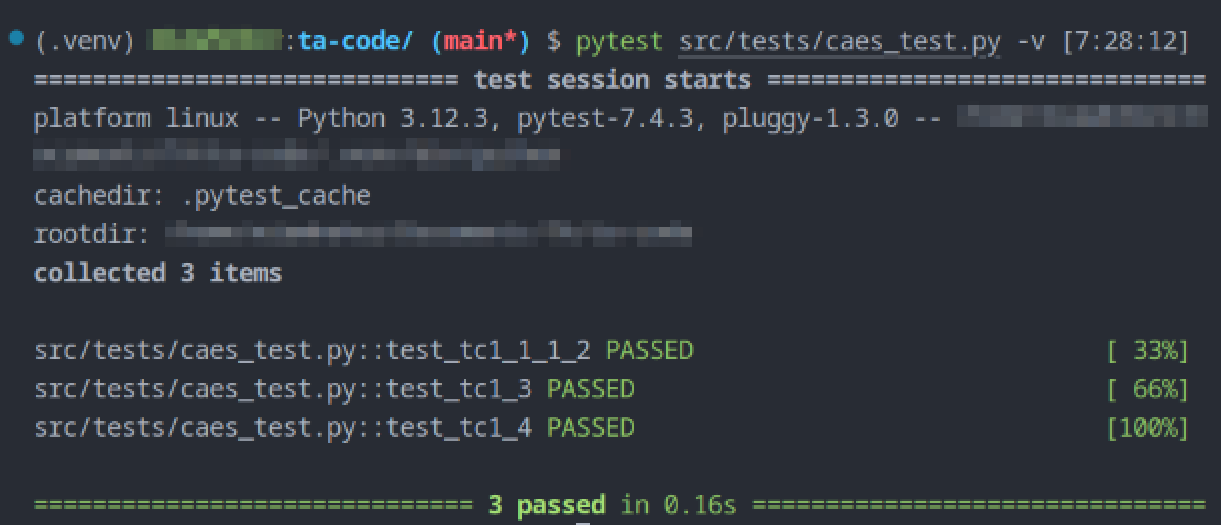
\includegraphics[width=0.8\textwidth]{chapters/res/appendix-3/result.png}
  \caption{Hasil Pengujian Skenario}
  \label{fig:skenario}
\end{figure}